% Dokumentenklasse: 
%   - {article} : für Kurzberichte.
% Dokumentenklasseoptionen:
%   - [11pt]    : Schriftgröße
%   - [a4paper] : Seitenformat DIN A4
%   - [twoside] : zweiseitig bedruckt
%   - [fleqn]   : linksbündige Ausrichtung der Gleichungen
\documentclass[11pt, a4paper, twoside, fleqn]{article}
% Das Paket inputenc erlaubt die direkte Eingabe von Sonderzeichen wie zum Beispiel deutschen Umlauten, um deren Trennung zu ermöglichen wird zudem das Paket fontenc mit eingebunden.
\usepackage[utf8]{inputenc}
\usepackage[T1]{fontenc}
% Hierbei wird ngerman als Option des Paketes babel gesetzt.
\usepackage[ngerman]{babel}
% Mit fullpage kann die Texthöhe und -breite sowie die Ränder festlegen, dass die Seite fast voll ist.
\usepackage{fullpage}
\usepackage{amsmath, amssymb}
\usepackage{multicol}
% Mit xcolor können Seiten, die Schrift, Rahmen und Felder in den verfügbaren Farben gesetzt werden.
\usepackage{xcolor}
\usepackage{tikz}
% Anpassbare Enumerates/Itemizes
\usepackage{enumitem}
\usepackage{graphicx}
\setlength{\mathindent}{0cm}
\setlength\parindent{0pt}
\setlength{\parskip}{0em}
\renewcommand{\baselinestretch}{1.2}
\graphicspath{{./images/}}
\title{Stromarten} 
\author{Ioannis Christodoulakis}
\date{\today}
\begin{document}
% Der Befehl \selectlanguage{ngerman} ändert die Standardsprache des Dokumentes.
\selectlanguage{ngerman}
\maketitle
% Die Anweisung beendet lediglich die aktuelle Seite.
\newpage
% Dieser Befehl veranlasst LaTeX ein Inhaltsverzeichnis zu erzeugen. 
\tableofcontents
% Die Anweisung beendet lediglich die aktuelle Seite.
\newpage
%%%%%%%%%%%%%%%%%%%%%%%%%%%%%%%%%%%%%%%%%%%%%%%%%%%%%%%%%%%%%%%%%%%%%%%%%%%%%%%%%%%%%%%%%%%%%%%%%%%%
%%%%%%%%%%%%%%%%%%%%%%%%%%%%%%%%%%%%%%%%%%%%%%%%%%%%%%%%%%%%%%%%%%%%%%%%%%%%%%%%%%%%%%%%%%%%%%%%%%%%
\section{Stromarten}
Grundsätzlich unterscheiden wir 3 Stromarten:
\subsection{Gleichstrom (DC)}
\begin{flushleft}
In einem Stromkreis fliesst ein Gleichstrom, wenn sich in einer bestimmten Zeit gleich viele Elektronen in die gleiche Richtung bewegen. Gleichstrom fliesst nur in eine Richtung mit gleich bleibender Stromstärke. Entsteht z.B. durch Batterien und Akkumulatoren (Akkus).
\end{flushleft}
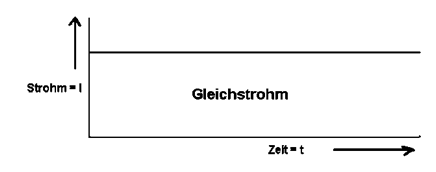
\includegraphics[scale=0.6]{DC_Strom}
\subsection{Wechselstrom (AC)}
\begin{flushleft}
Im Stromkreis fliesst Wechselstrom, wenn sich Elektronen in einem Leiter hin und zurück bewegen. Im Diagramm erhalten wir eine Sinuslinie. Dieser Wechselstrom fliesst immer in wechselnder Richtung und Stärke, 50 Mal in der Sekunde. Diese Wechselfrequenz nennt man Hertz. Im normalen Stromnetz fliesst Wechselstrom. Wechselstrom entsteht z.B. durch Generatoren, Transformatoren.
\end{flushleft}
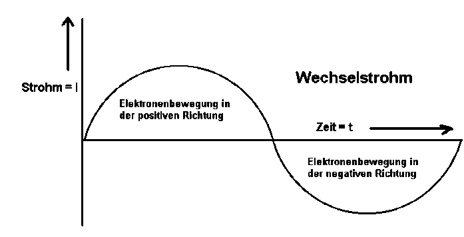
\includegraphics[scale=0.6]{AC_Strom}
\subsection{Mischstrom}
\begin{flushleft}
Mischstrom setzt sich zusammen aus einem Gleichstromanteil und einem Wechselstromanteil. Er fliesst, genau wie der Gleichstrom immer in dieselbe Richtung, bleibt in seiner Grösse aber nicht konstant.
\end{flushleft}
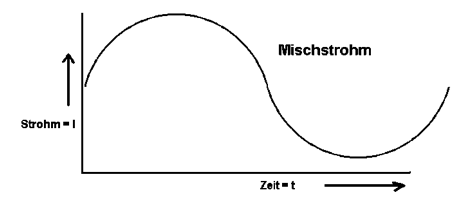
\includegraphics[scale=0.6]{Misch_Strom}
\end{document}